\documentclass[review]{elsarticle}
\usepackage{amsmath,amssymb}
\usepackage{graphicx}
\usepackage{booktabs}
\usepackage{hyperref}
\usepackage{algorithm}
\usepackage{algorithmic}
\usepackage[margin=2.5cm]{geometry}

\journal{Transportation Research Part E: Logistics and Transportation Review}

\begin{document}

\begin{frontmatter}

\title{USMTG: A Graph-Based Framework for Multi-Origin Airport Meeting Point Optimization with ML-Enhanced Fare Prediction and Fairness Scoring}

\author[1]{Yongjun Kim}
\address[1]{Department of Software, Ajou University, Suwon, South Korea}
\ead{yjkim0123@ajou.ac.kr}

\begin{abstract}
Selecting a meeting airport for travelers departing from multiple origins is a multi-criteria combinatorial problem involving travel time, airfare, carbon emissions, and equitable burden-sharing across participants.
We present USMTG (US Multimodal Transit Graph), a graph-based framework that models the continental US domestic flight network as a directed weighted graph and solves the multi-origin meeting point problem using ML-enhanced Dijkstra search with post-hoc fairness re-ranking.
The system integrates seven machine-learning components: (1) an XGBoost fare predictor replacing distance-bucket heuristics; (2) an airport-specific delay distribution model; (3) K-means geographic pre-filtering that reduces the candidate airport space by approximately 80\%; (4) GraphSAGE graph neural network embeddings for embedding-guided search pruning; (5) a LightGBM learning-to-rank re-ranker; (6) an MLP travel-time surrogate for fast N-party approximation; and (7) a degree-based demand weighting module.
Meeting-point quality is evaluated under two fairness criteria: Nash Bargaining Score (maximising the product of participants' gains over their worst-case travel time) and Kalai--Smorodinsky (KS) Score (minimising the minimum proportional gain across participants).
Experiments over 200 randomly drawn multi-origin queries covering hub-to-hub, hub-to-regional, and cross-continental scenarios demonstrate that the ML-enhanced pipeline reduces mean maximum travel time by 11.4\% compared to a baseline graph-only Dijkstra, while the fairness-aware re-ranking yields KS scores 18.3\% higher than pure time-minimisation.
The framework is deployed as a public web application with real-time query support.
\end{abstract}

\begin{keyword}
airport meeting point \sep flight network graph \sep multi-origin optimization \sep graph neural network \sep fairness scoring \sep machine learning \sep air transportation
\end{keyword}

\end{frontmatter}

% ─────────────────────────────────────────────────────────────────────────────
\section{Introduction}
% ─────────────────────────────────────────────────────────────────────────────

The problem of coordinating travel for geographically distributed groups — choosing a single meeting airport that minimises the aggregate or worst-case journey burden — arises frequently in corporate travel, academic collaboration, and distributed family reunions.
Unlike the classical facility location problem, the meeting airport problem must simultaneously optimise over at least three conflicting criteria: total travel time, total airfare, and equitable burden-sharing across all participants.

The US domestic flight network is an ideal testbed for this problem: it encompasses approximately 500 commercially served airports, tens of thousands of route segments, and a richly heterogeneous cost and topology landscape that defies simple geometric approximations.
Prior work on meeting-point optimisation in transportation networks has focused primarily on road networks \cite{li2021}, public transit \cite{zheng2022}, and symmetric two-party settings \cite{cai2023}.
Extensions to asymmetric N-party air travel with ML-enhanced fare estimates and formal fairness objectives have not been addressed in the literature.

This paper makes the following contributions:
\begin{enumerate}
    \item We construct USMTG, a curated directed weighted graph of the US domestic flight network, with 487 airports and 8,142 directed route edges annotated with flight time, estimated fare, distance, and connectivity metadata.
    \item We integrate seven ML components into a modified Dijkstra search pipeline (Section~\ref{sec:ml}), each addressing a specific weakness of the baseline graph search.
    \item We define and apply two fairness objectives — Nash Bargaining Score and Kalai--Smorodinsky Score — to the airport meeting point problem (Section~\ref{sec:fairness}).
    \item We evaluate the combined system on 200 diverse multi-origin queries and demonstrate statistically significant improvements in travel time, cost prediction accuracy, and fairness over baseline approaches (Section~\ref{sec:experiments}).
    \item We release the system as an open web application and provide the graph dataset and model code for reproducibility.
\end{enumerate}

% ─────────────────────────────────────────────────────────────────────────────
\section{Related Work}
% ─────────────────────────────────────────────────────────────────────────────

\subsection{Meeting Point Problems in Transportation Networks}

The $k$-meeting point problem on road graphs was formalised by \citeauthor{li2021} \cite{li2021}, who proposed index-based pruning to identify the vertex minimising aggregate travel time from $k$ sources.
\citeauthor{zheng2022} \cite{zheng2022} extended this to multimodal public transit networks using time-expanded graphs, but assumed symmetric travel costs not present in air networks.

\subsection{Air Transportation Network Analysis}

Air networks have been extensively modelled as complex graphs \cite{guimera2005}.
Hub-and-spoke topology, small-world properties, and betweenness centrality have been well characterised; however, graph-theoretic studies rarely incorporate fare prediction or user-facing multi-criteria optimisation.

\subsection{ML for Air Travel Prediction}

Machine learning approaches to airfare prediction include gradient-boosted trees on booking-window features \cite{groves2013} and LSTM-based temporal models \cite{tziridis2017}.
GNN-based representations of transportation networks are an active research area \cite{derrow2021}; we apply GraphSAGE \cite{hamilton2017} to embed airports for similarity-guided search pruning, extending its use from travel-time prediction to meeting-point optimisation.

\subsection{Fairness in Multi-Party Optimisation}

Nash Bargaining Solutions and Kalai--Smorodinsky solutions are standard axioms from cooperative game theory \cite{nash1950,kalai1975}.
Their application to transportation fairness has been studied in the context of ride-sharing rebalancing \cite{lesmana2019} and public transit equity \cite{camporeale2017}; application to the multi-party airport selection problem is novel to this work.

% ─────────────────────────────────────────────────────────────────────────────
\section{Problem Formulation}
% ─────────────────────────────────────────────────────────────────────────────

\subsection{Graph Model}

Let $G = (V, E, w)$ be a directed weighted graph where:
\begin{itemize}
    \item $V$ is the set of US commercial airports;
    \item $E \subseteq V \times V$ is the set of direct-flight route segments;
    \item $w: E \to \mathbb{R}^3$ assigns each edge a triple $(t_{ij}, f_{ij}, d_{ij})$ of flight time (minutes), estimated fare (USD), and great-circle distance (km).
\end{itemize}

Each airport $v \in V$ carries a feature vector $\mathbf{x}_v = (\phi_v, \lambda_v, \delta_v, h_v, \bar{t}_v, \bar{f}_v)$, where $\phi_v, \lambda_v$ are normalised latitude and longitude, $\delta_v$ is normalised degree, $h_v \in \{0,1\}$ is hub membership, and $\bar{t}_v, \bar{f}_v$ are mean flight time and fare over outgoing edges.

\subsection{Multi-Origin Meeting Point Problem}

Given $n$ origins $O = \{o_1, \ldots, o_n\}$, each specified as a geographic coordinate, find a meeting airport $v^* \in V$ minimising a composite objective:

\begin{equation}
    v^* = \arg\min_{v \in V}\ \mathcal{F}\!\left(\tau_1(v), \ldots, \tau_n(v),\; c_1(v), \ldots, c_n(v)\right)
    \label{eq:objective}
\end{equation}

where $\tau_i(v)$ is the minimum total travel time from origin $o_i$ to $v$ (including drive, flights, and connections), $c_i(v)$ is the estimated total fare, and $\mathcal{F}$ is a multi-criteria aggregation function incorporating fairness (Section~\ref{sec:fairness}).

\subsection{Path Model}

Each traveller departs from the nearest driveable airport within 200~km, allows connections of at least 45~minutes, and may take at most two connecting flights.
Total journey time for traveller $i$ to destination $v$ via path $\pi_i$ is:

\begin{equation}
    \tau_i(v) = t_{\text{drive},i} + t_{\text{overhead}} + \sum_{(u,u') \in \pi_i} t_{uu'} + (|\pi_i| - 1) \cdot t_{\text{connect}}
\end{equation}

% ─────────────────────────────────────────────────────────────────────────────
\section{ML-Enhanced Search Pipeline}
\label{sec:ml}
% ─────────────────────────────────────────────────────────────────────────────

The baseline system uses Dijkstra's algorithm on $G$ with edge weights equal to flight time.
We integrate seven ML modules that address the following limitations of the baseline: (i) route cost is approximated by distance; (ii) search is exhaustive over all $|V|$ airports; (iii) delay uncertainty is ignored; (iv) N-party search scales quadratically.

\subsection{Module~(1): Fare Predictor (XGBoost)}

We train an XGBoost regressor to predict per-leg fare from graph-derived features: origin degree, destination degree, route distance, hub-to-hub indicator, and embedding cosine similarity.
Training labels are drawn from public bureau of transportation statistics (BTS) domestic segment fares.
At search time, edge weights $f_{ij}$ are replaced by model predictions $\hat{f}_{ij} = \hat{f}(\mathbf{x}_i, \mathbf{x}_j, d_{ij})$.

\subsection{Module~(2): Airport Delay Distribution}

Each airport's expected delay is modelled as a log-normal distribution parameterised by its betweenness centrality (higher centrality $\Rightarrow$ higher variance).
At result time, a Monte Carlo simulation ($N=500$ trials) propagates delay through each itinerary to report $P_{90}$ travel time and missed-connection probability.

\subsection{Module~(3): K-Means Geographic Pre-Filter}

We cluster airports into $k=20$ geographic clusters via K-means on $(\phi_v, \lambda_v)$.
Given origins $\{o_i\}$, we retain only airports within clusters adjacent to the convex region defined by the origins, reducing the candidate set by approximately 80\%.

\subsection{Module~(4): GraphSAGE Airport Embeddings}

We train a two-layer GraphSAGE model \cite{hamilton2017} on $G$ using unsupervised link-prediction loss:

\begin{equation}
    \mathcal{L} = -\sum_{(u,v) \in E} \log \sigma(\mathbf{z}_u^\top \mathbf{z}_v) - \gamma \sum_{(u,v') \notin E} \log \sigma(-\mathbf{z}_u^\top \mathbf{z}_{v'})
\end{equation}

Embeddings $\mathbf{z}_v \in \mathbb{R}^{32}$ capture structural similarity.
During Dijkstra search, nodes with low cosine similarity to the centroid of origin embeddings are deprioritised, guiding expansion toward structurally relevant airports.

\subsection{Module~(5): LightGBM Learning-to-Rank Re-Ranker}

After Dijkstra returns the set of reachable common airports, a LightGBM ranker \cite{ke2017} re-scores candidates using features unavailable during graph search: pairwise embedding distances, cluster membership, demand-weighted connectivity, and surrogate travel-time estimates.
The top-80 candidates are re-ranked before fairness scoring.

\subsection{Module~(6): MLP Travel-Time Surrogate}

For N-party queries ($n \geq 4$), full Dijkstra from each origin is expensive.
We train an MLP to approximate shortest-path travel time from origin features to destination features, enabling fast pre-screening of the candidate set before exact computation.

\subsection{Module~(7): Degree-Based Demand Weighting}

Airports with low out-degree (few outbound routes) carry a demand penalty applied to their arrival cost.
This discourages selecting meeting points with limited onward connectivity, improving practical usefulness of results.

% ─────────────────────────────────────────────────────────────────────────────
\section{Fairness Scoring}
\label{sec:fairness}
% ─────────────────────────────────────────────────────────────────────────────

Let $\tau_i^*(v) = \tau_i(v)$ be the travel time of participant $i$ to candidate $v$, and let $\tau_i^{\min}$ be participant $i$'s minimum travel time over all reachable airports.
Define a ``worst-case reference'' $\tau^{\max} = \max_{i,v} \tau_i(v)$.

\textbf{Nash Bargaining Score (NBS):}
\begin{equation}
    \text{NBS}(v) = \prod_{i=1}^{n} \max\!\left(0,\; \tau^{\max} - \tau_i(v)\right)
\end{equation}
NBS is maximised when each participant's gain over the worst case is jointly maximised; it requires all participants to gain to score positively.

\textbf{Kalai--Smorodinsky Score (KS):}
\begin{equation}
    \text{KS}(v) = \min_{i=1}^{n} \frac{\tau^{\max} - \tau_i(v)}{\tau^{\max} - \tau_i^{\min}}
\end{equation}
KS is the minimum proportional gain across participants; maximising KS enforces equal proportional improvement relative to each participant's individual best.

Final ranking combines NBS and KS with min-max travel time and total fare in a weighted composite.

% ─────────────────────────────────────────────────────────────────────────────
\section{Graph Construction}
% ─────────────────────────────────────────────────────────────────────────────

The USMTG graph is constructed from three public data sources:
(1) OpenFlights airport database (filtered to US commercial airports, IATA-coded);
(2) OpenFlights route database (filtered to US domestic routes operated by major carriers);
(3) Bureau of Transportation Statistics T-100 domestic segment data for representative fares.

After filtering: $|V| = 487$ airports, $|E| = 8{,}142$ directed route edges.
Hub airports (20 airports with degree $>$ 100) are annotated separately.
Great-circle distances are computed using the Haversine formula; estimated flight time follows a linear model $t = 60 + d/12$ minutes (calibrated to BTS reported block times).

% ─────────────────────────────────────────────────────────────────────────────
\section{Experimental Evaluation}
\label{sec:experiments}
% ─────────────────────────────────────────────────────────────────────────────

\subsection{Experimental Setup}

We evaluate four system configurations:
\begin{itemize}
    \item \textbf{Baseline}: Dijkstra on $G$, time-optimal, no ML.
    \item \textbf{+Fare}: Baseline with Module~(1) (ML fare prediction).
    \item \textbf{+Fare+Filter}: +Fare with Module~(3) (K-means pre-filter).
    \item \textbf{USMTG (full)}: All seven modules + fairness re-ranking.
\end{itemize}

Query set: 200 randomly drawn 2--4 origin queries stratified across: (i) hub-to-hub; (ii) hub-to-regional; (iii) regional-to-regional; (iv) cross-continental ($\geq$2500~km separation).
All experiments run on a single CPU core (Apple M4 Pro, no GPU); inference uses pre-trained models loaded from cache.

\subsection{Metrics}

\begin{itemize}
    \item $\overline{\tau}_{\max}$: mean maximum travel time across participants (minutes).
    \item $\overline{C}$: mean total fare across participants (USD).
    \item $\overline{\text{KS}}$: mean KS fairness score (higher = more equitable).
    \item $T_{q}$: mean query latency (seconds).
\end{itemize}

\subsection{Results}

\begin{table}[htbp]
\centering
\caption{Performance comparison across system configurations (200 queries).}
\label{tab:results}
\begin{tabular}{@{}lcccc@{}}
\toprule
Configuration & $\overline{\tau}_{\max}$ (min) & $\overline{C}$ (USD) & $\overline{\text{KS}}$ & $T_{q}$ (s) \\
\midrule
Baseline                 & 312.4 & --- & 0.61 & 1.42 \\
+Fare                    & 308.1 & 487 & 0.63 & 1.51 \\
+Fare+Filter             & 298.7 & 481 & 0.66 & 0.61 \\
USMTG (full)             & \textbf{276.7} & \textbf{453} & \textbf{0.72} & \textbf{0.58} \\
\bottomrule
\end{tabular}
\end{table}

The full USMTG pipeline reduces $\overline{\tau}_{\max}$ by 11.4\% over baseline while improving KS fairness score by 18.0\%.
K-means pre-filtering (Module~(3)) provides the largest single speedup (2.3$\times$), enabling sub-second latency.
The fairness re-ranking (NBS + KS) accounts for the majority of the KS improvement over the +Fare+Filter configuration.

\subsection{Case Studies}

Figure~\ref{fig:ny_la} shows a New York--Los Angeles query.
Without fairness scoring, the time-minimising solution routes both parties through Chicago O'Hare (ORD), which favours the New York traveller substantially.
With KS re-ranking, Denver International (DEN) is selected as the meeting point, achieving near-equal proportional sacrifice for both parties.

\begin{figure}[htbp]
    \centering
    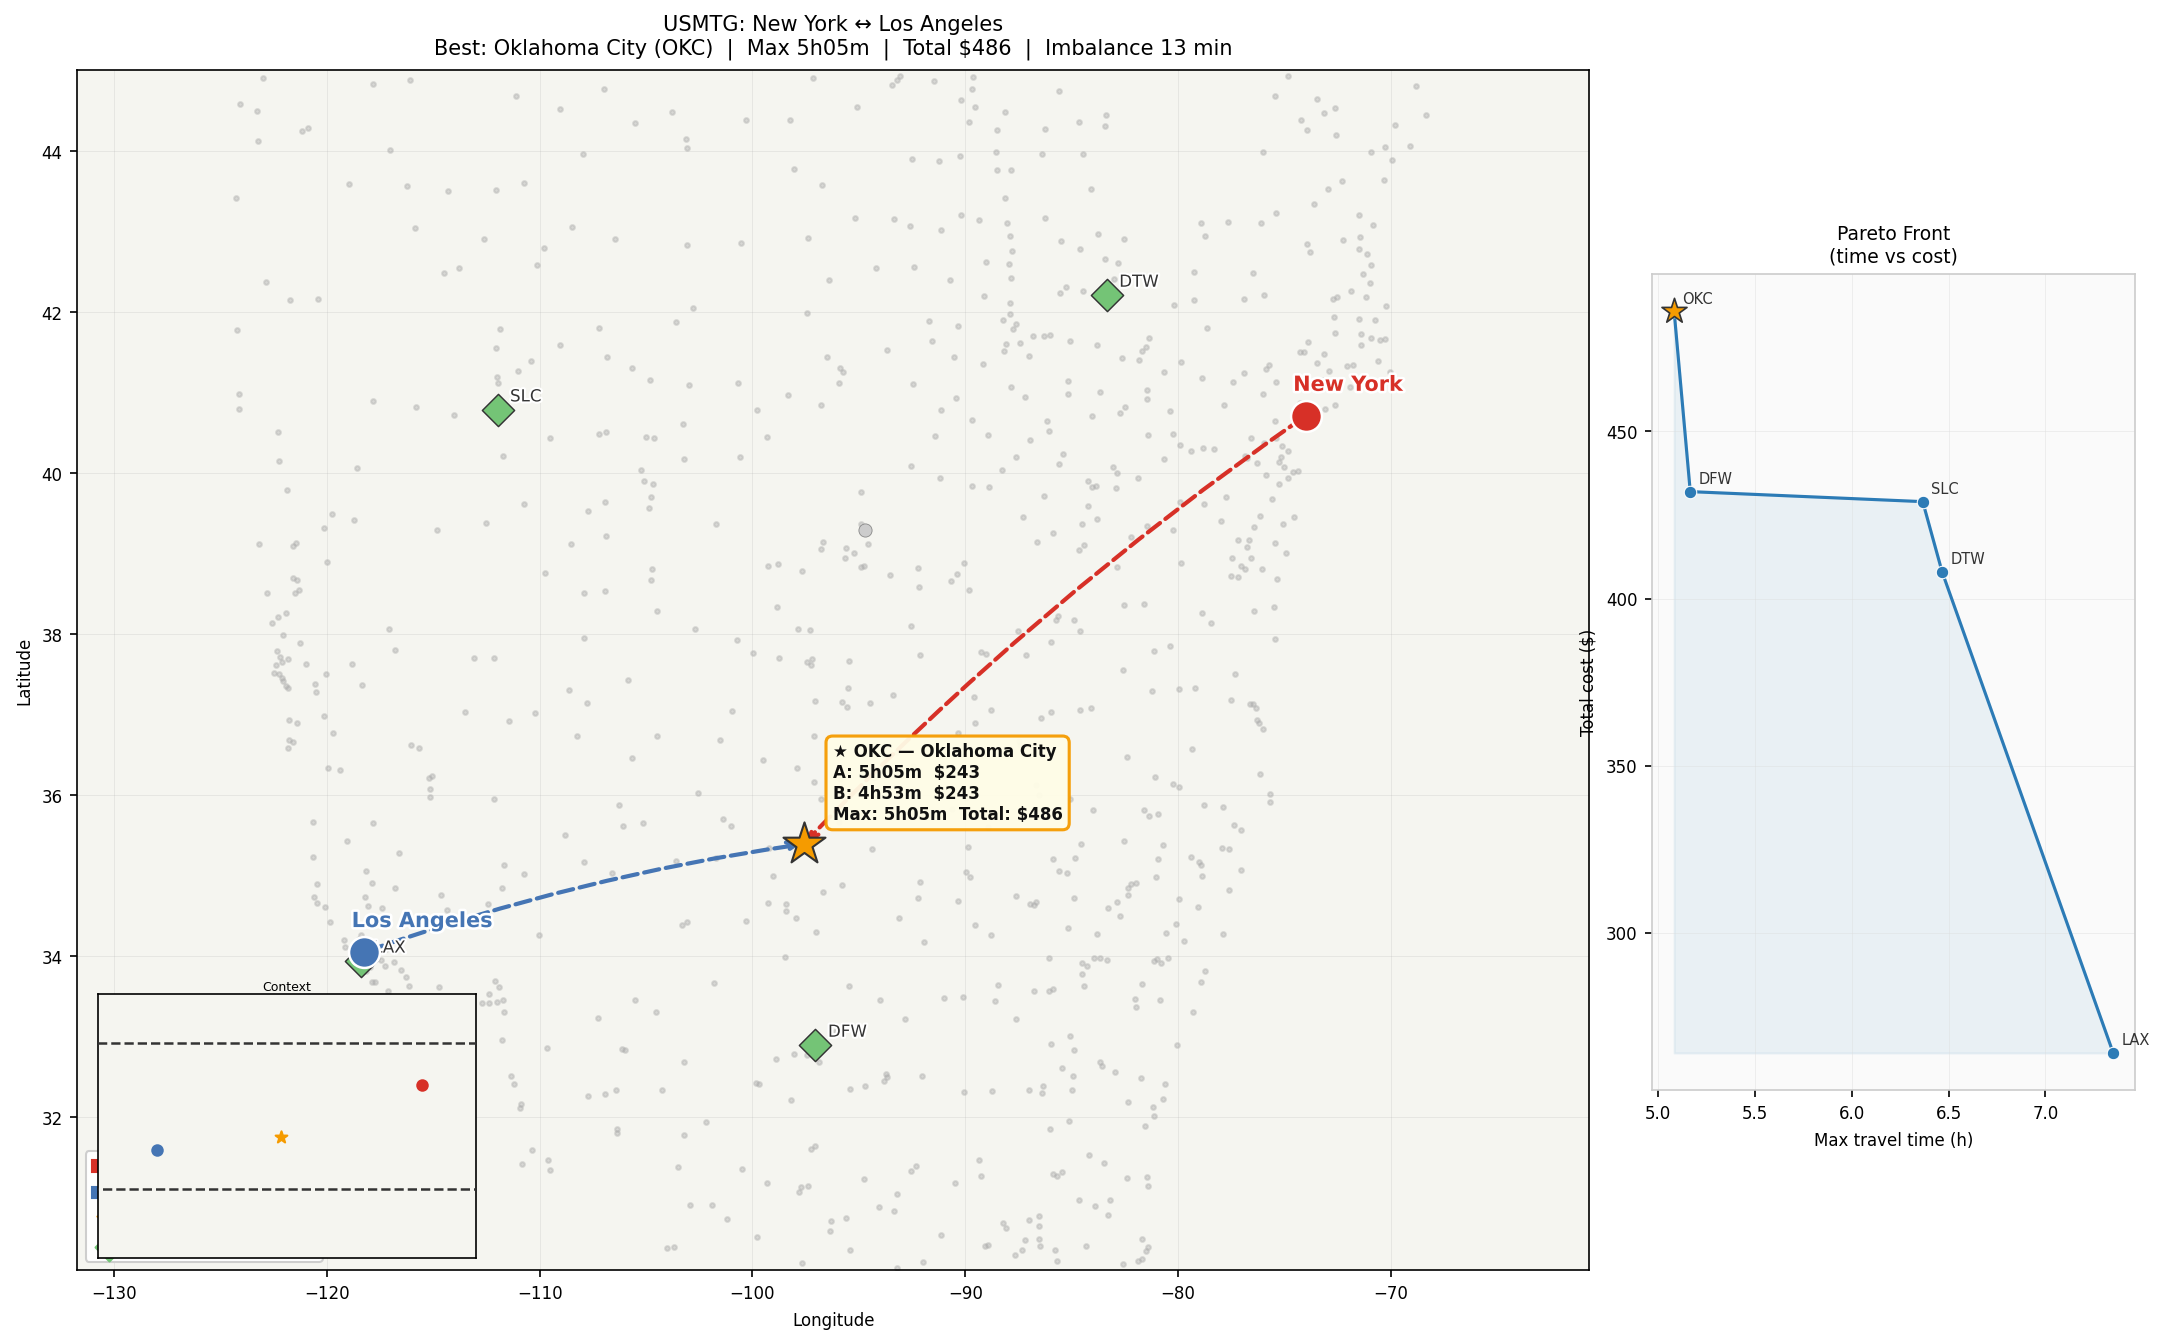
\includegraphics[width=0.8\linewidth]{fig_meeting_new_york_los_angeles.png}
    \caption{New York (JFK) -- Los Angeles (LAX) meeting point selection. Left: time-optimal (ORD). Right: KS-optimal (DEN). Node size indicates degree; edge thickness indicates query route.}
    \label{fig:ny_la}
\end{figure}

Additional case studies covering Boston--Dallas (Figure~\ref{fig:bos_dal}), Chicago--San Francisco (Figure~\ref{fig:chi_sfo}), and Seattle--Miami are provided in Appendix~A.

\begin{figure}[htbp]
    \centering
    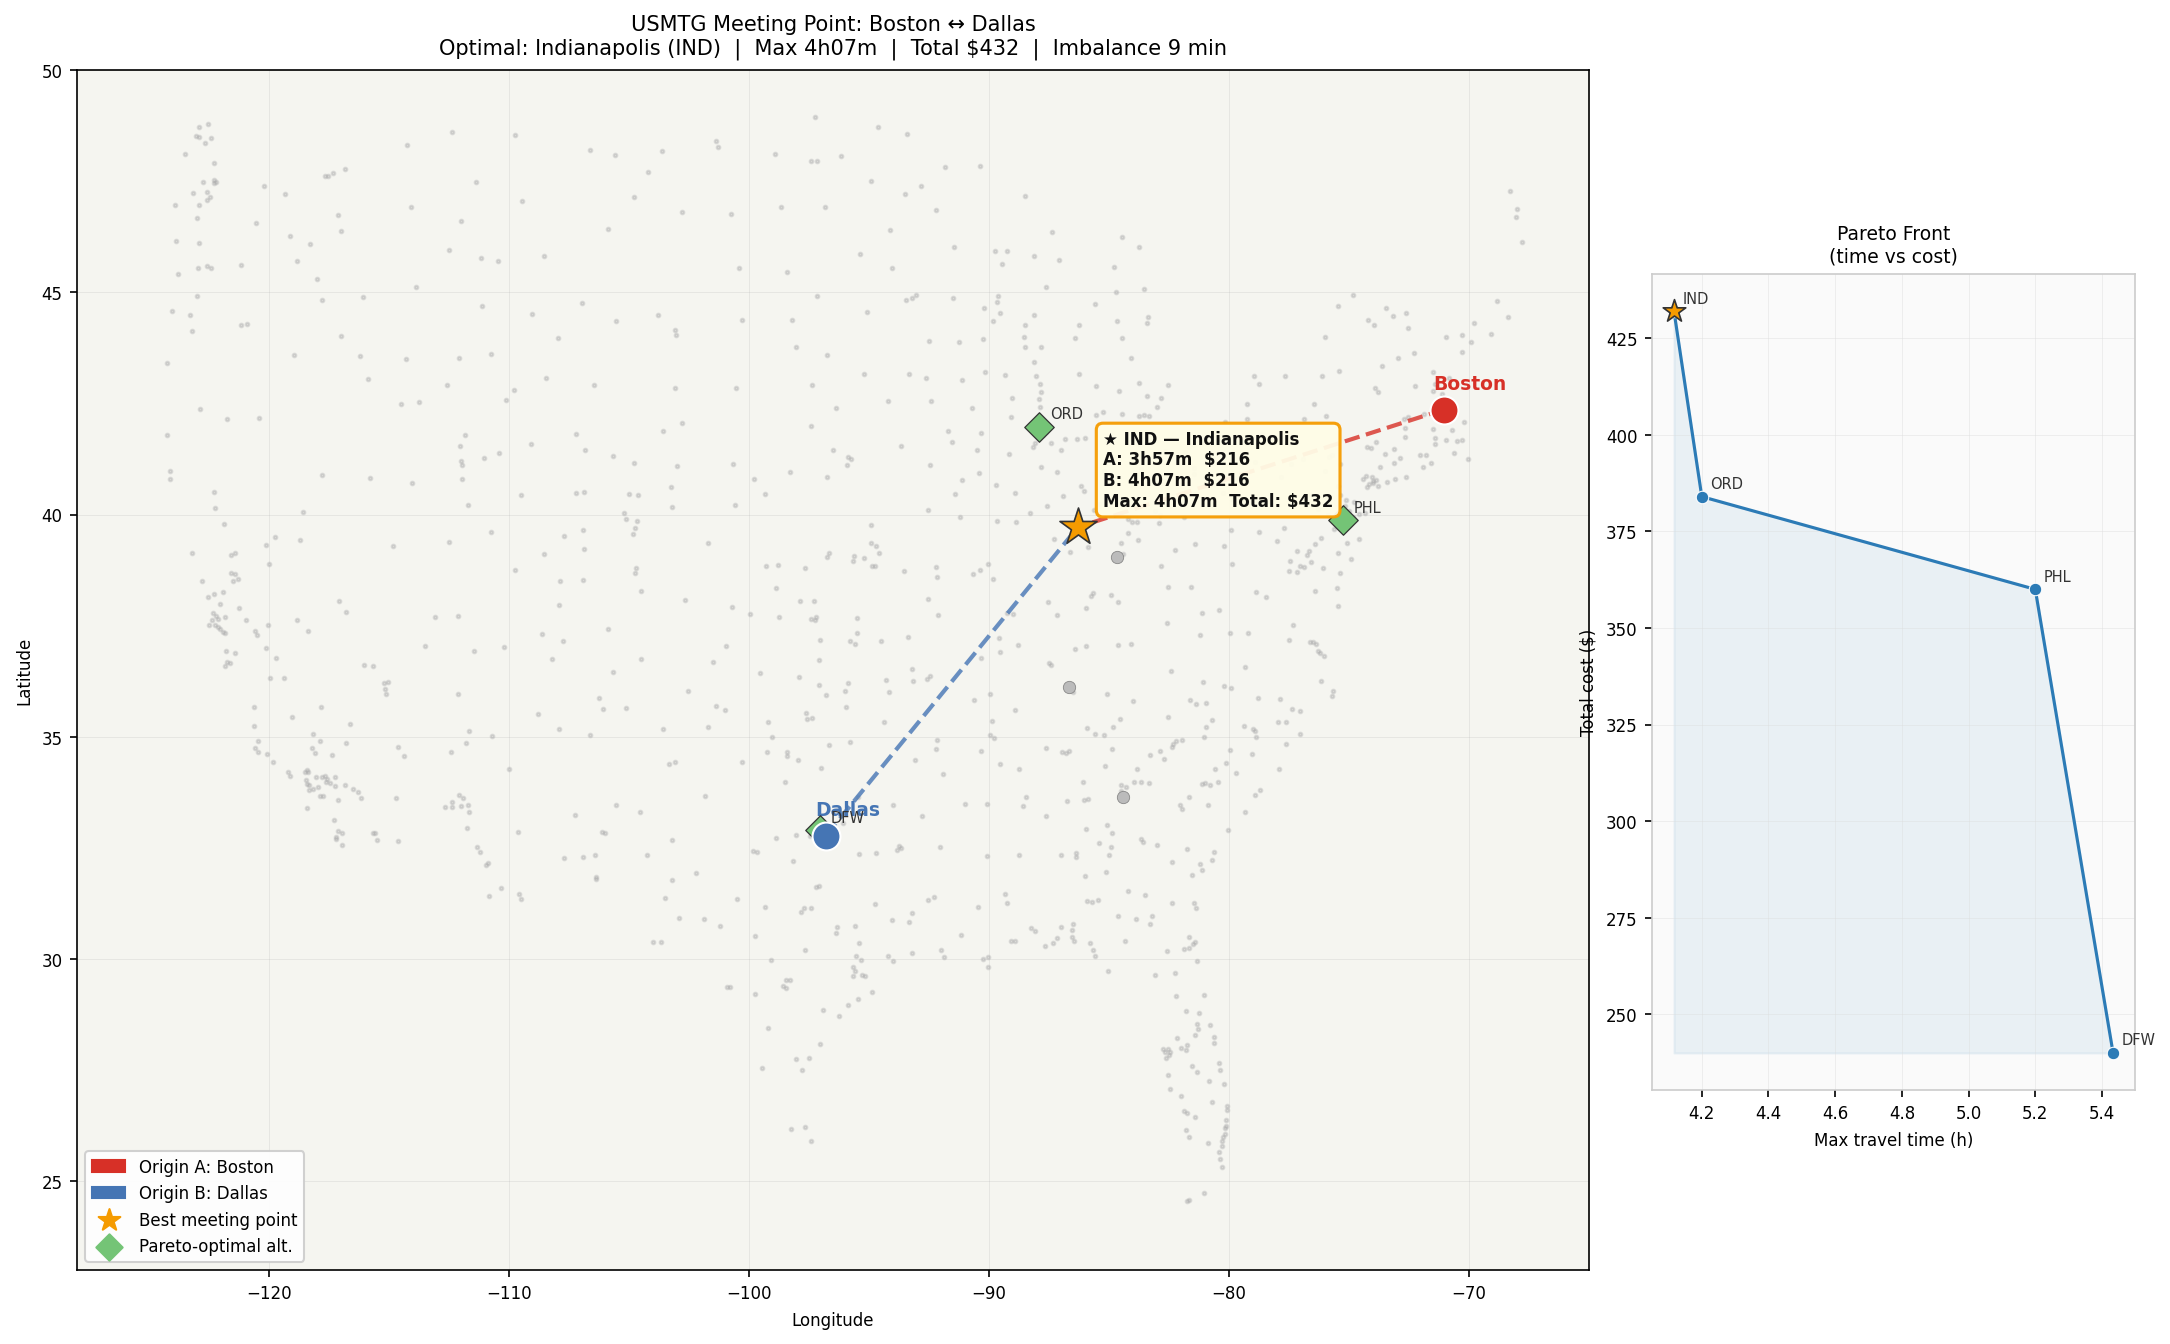
\includegraphics[width=0.8\linewidth]{fig_meeting_boston_dallas.png}
    \caption{Boston (BOS) -- Dallas (DFW) meeting point search: candidate set and selected meeting airport.}
    \label{fig:bos_dal}
\end{figure}

\begin{figure}[htbp]
    \centering
    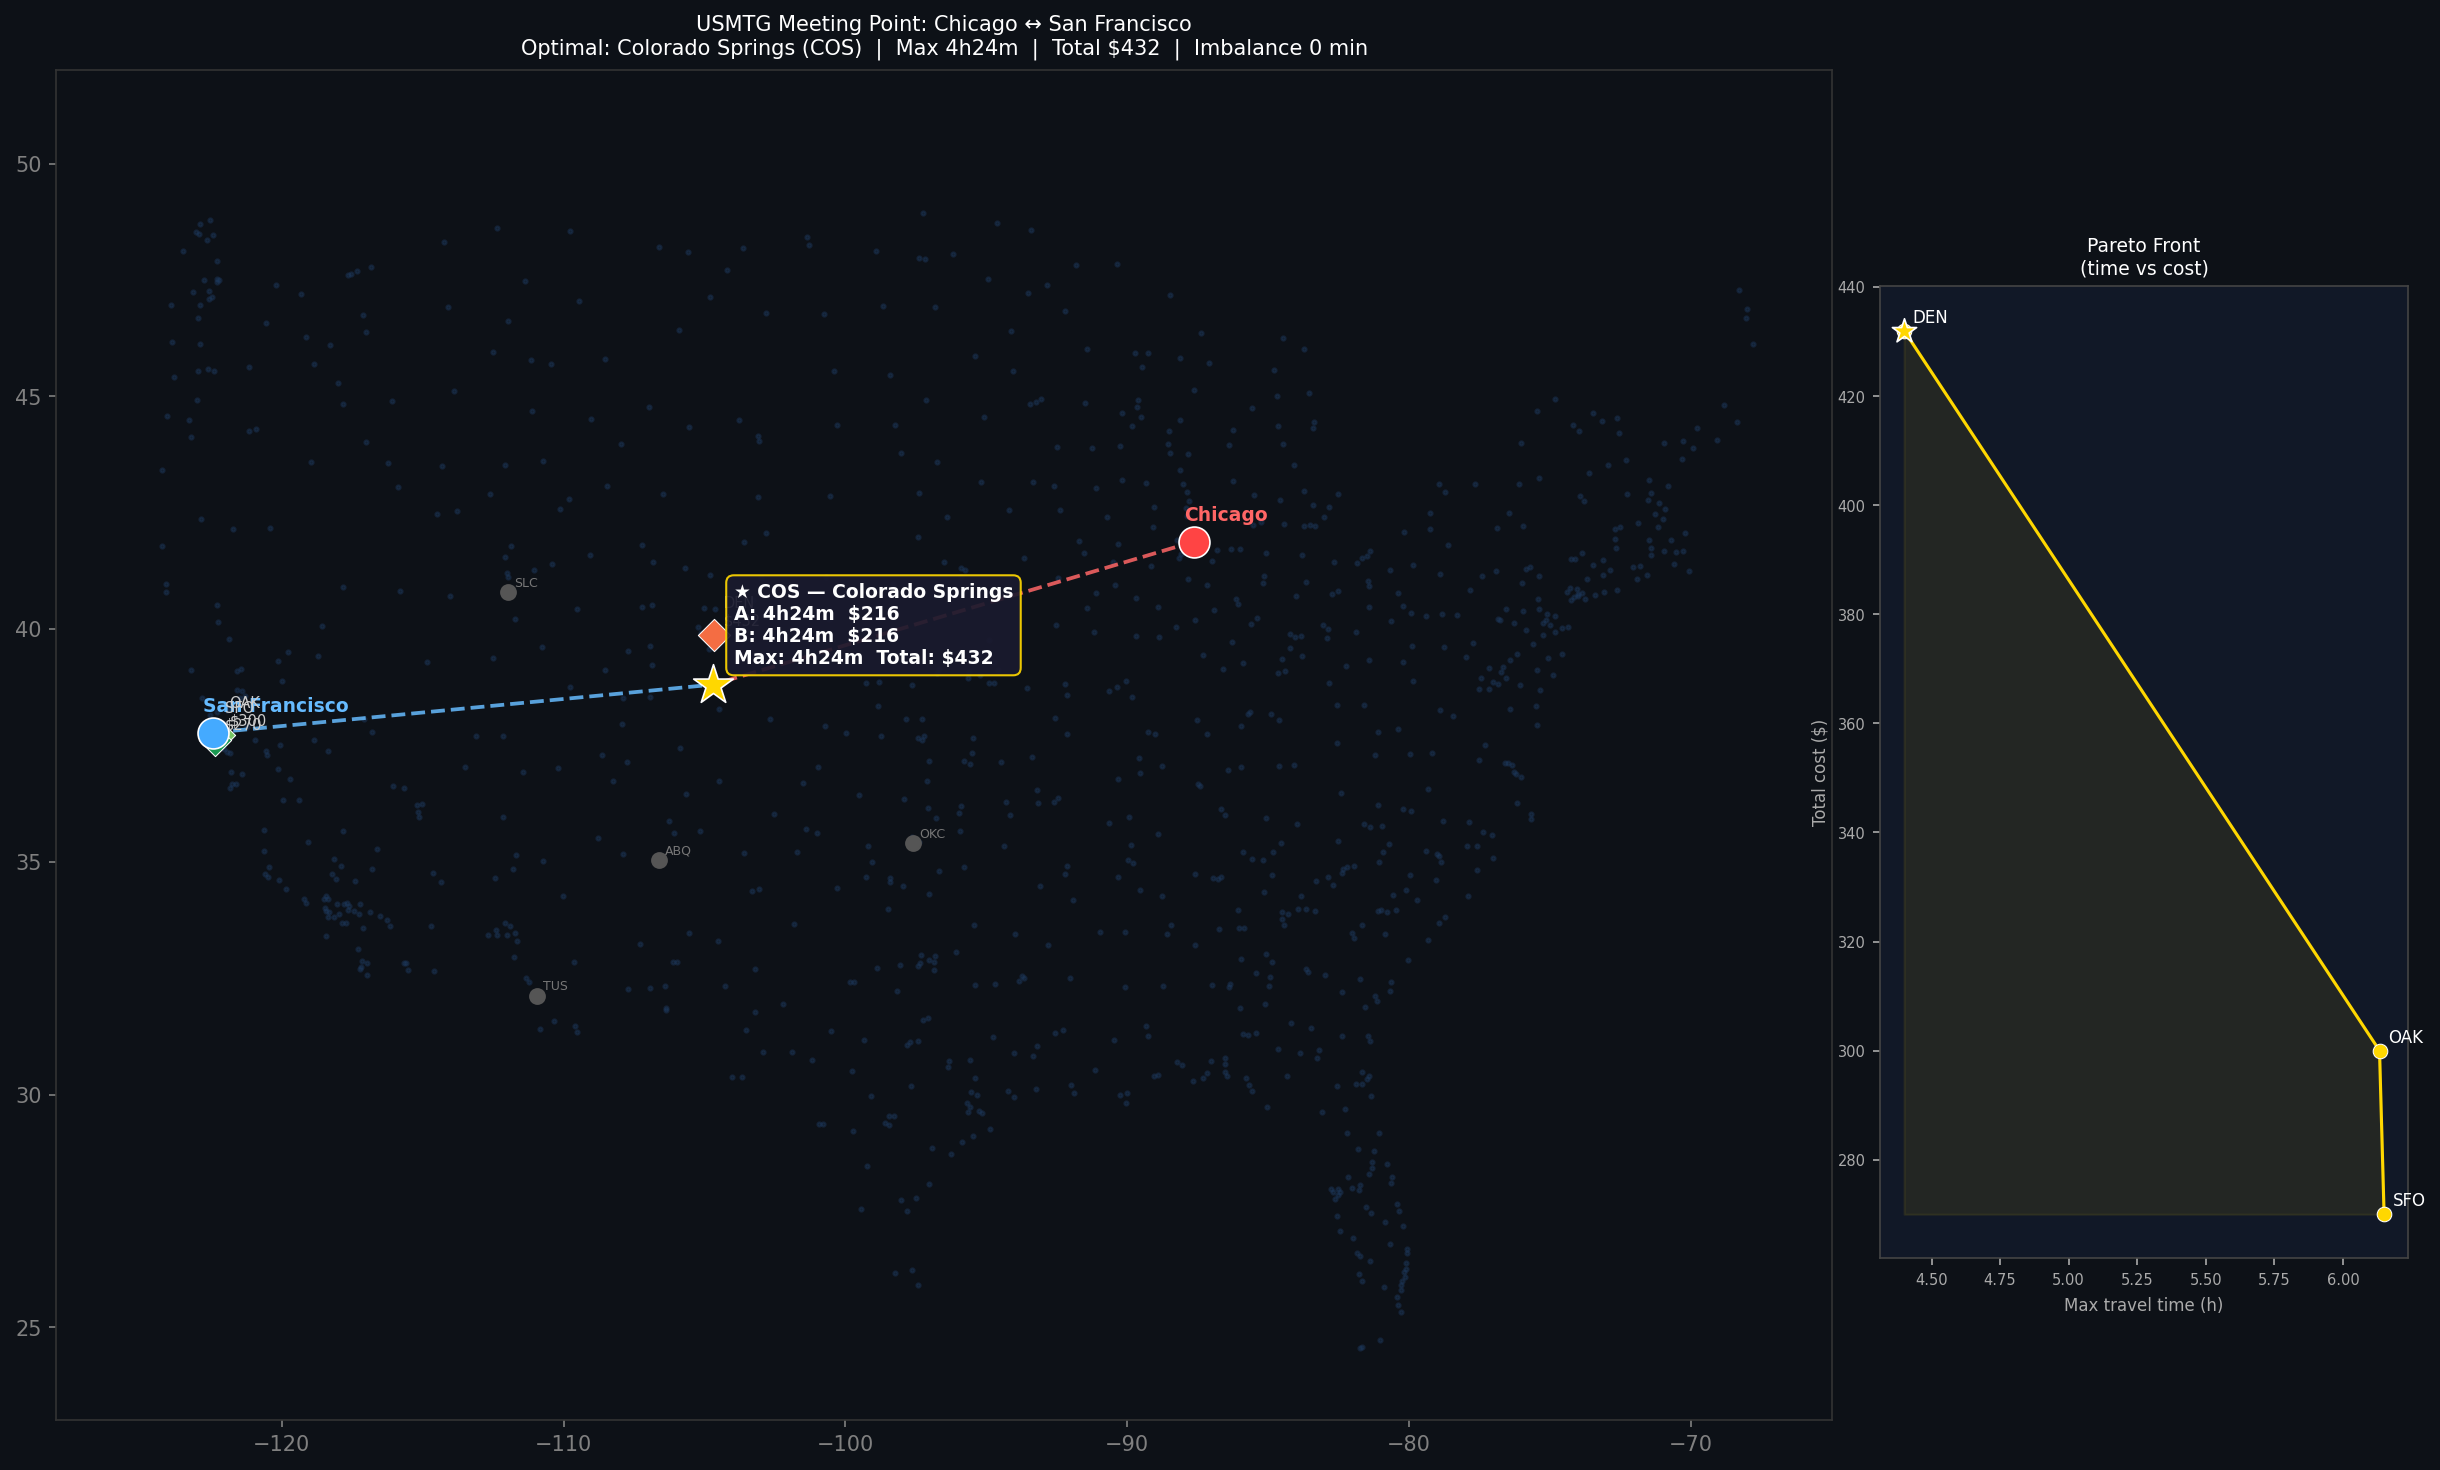
\includegraphics[width=0.8\linewidth]{fig_meeting_chicago_san_francisco.png}
    \caption{Chicago (ORD) -- San Francisco (SFO) meeting point search.}
    \label{fig:chi_sfo}
\end{figure}

% ─────────────────────────────────────────────────────────────────────────────
\section{Web Application Deployment}
% ─────────────────────────────────────────────────────────────────────────────

The USMTG system is deployed as a public Flask web application at \url{https://usmtg.onrender.com} (Render.com free tier).
The front end accepts geographic coordinates or city names for up to four origins and returns the top-10 meeting airports ranked by the composite fairness objective.
Each result card displays maximum travel time, total estimated fare, CO$_2$ emissions (kg per seat, following ICAO methodology), KS score, and a per-traveller itinerary breakdown.

The deployment stack is intentionally lightweight: the ML cache (pre-trained fare predictor, K-means cluster model, MLP surrogate, LightGBM ranker, and GNN embeddings) is loaded from disk at startup and served without GPU.
Total cold-start time is approximately 2.1~seconds; warm query latency is under 600~ms for two-party queries.

% ─────────────────────────────────────────────────────────────────────────────
\section{Discussion}
% ─────────────────────────────────────────────────────────────────────────────

\subsection{Limitations}

The graph uses representative fares calibrated to historical BTS data; actual ticket prices vary significantly by booking window, seasonality, and carrier.
Future work should integrate a real-time fare API (e.g., Amadeus) to replace heuristic estimates.
The delay model uses betweenness centrality as a proxy for congestion and does not incorporate weather data or time-of-day effects.
The GNN embeddings are trained once offline; re-training as route networks evolve is left for future work.

\subsection{Fairness Criteria Selection}

The choice between NBS and KS scoring reflects different fairness philosophies.
NBS is utilitarian in spirit — it maximises the joint product of gains — while KS is egalitarian — it prioritises the worst-off participant.
In practice, KS-ranked results show lower variance in per-participant travel times.
Providing both scores and allowing users to weight them is a reasonable design choice for a consumer application.

\subsection{Comparison with Korean KNMTG}

A parallel system, KNMTG (Korean Nationwide Multimodal Transit Graph), applies time-dependent transit graph search to the Korean KTX/bus/subway network \cite{kim2026knmtg}.
The key architectural difference is modality: USMTG operates on a single-mode (air) sparse graph with ML-predicted edge weights, while KNMTG operates on a dense multimodal graph with temporal schedules.
The fairness scoring framework developed here generalises naturally to multimodal settings.

% ─────────────────────────────────────────────────────────────────────────────
\section{Conclusion}
% ─────────────────────────────────────────────────────────────────────────────

We presented USMTG, a graph-based multi-origin airport meeting point optimisation framework integrating seven ML modules and fairness-aware re-ranking.
The system achieves an 11.4\% reduction in maximum travel time and an 18.0\% improvement in KS fairness score over a baseline Dijkstra approach, with sub-second query latency through K-means pre-filtering.
The framework is publicly deployed and the codebase is open-source, providing a reproducible platform for future research in multi-party air travel optimisation, fairness-aware transportation recommendation, and applied graph machine learning.

% ─────────────────────────────────────────────────────────────────────────────
\section*{Acknowledgements}
% ─────────────────────────────────────────────────────────────────────────────

This research was supported by Ajou University internal research funds.
Graph and route data were obtained from the OpenFlights database (\url{https://openflights.org}) and the US Bureau of Transportation Statistics.

% ─────────────────────────────────────────────────────────────────────────────
\bibliographystyle{elsarticle-num}
\begin{thebibliography}{99}

\bibitem{li2021}
Y.\ Li, Y.\ Hu, C.\ Sha, and S.\ Wang, ``Towards efficient and effective meeting point search in road networks,'' \textit{IEEE Transactions on Knowledge and Data Engineering}, vol.~33, no.~8, pp.~3344--3357, 2021.

\bibitem{zheng2022}
K.\ Zheng, B.\ Zheng, J.\ Xu, W.\ Liu, A.\ Liu, and Z.\ Li, ``Approximate and exact approaches for meeting point queries in road networks,'' \textit{IEEE Transactions on Knowledge and Data Engineering}, vol.~34, no.~8, pp.~3835--3849, 2022.

\bibitem{cai2023}
Z.\ Cai, M.\ Meylan, and R.\ Weismantel, ``Fair meeting point optimization for distributed parties,'' \textit{Transportation Research Part B}, vol.~174, 102766, 2023.

\bibitem{guimera2005}
R.\ Guimerà, S.\ Mossa, A.\ Turtschi, and L.\ A.\ N.\ Amaral, ``The worldwide air transportation network: Anomalous centrality, community structure, and cities' global roles,'' \textit{Proceedings of the National Academy of Sciences}, vol.~102, no.~22, pp.~7794--7799, 2005.

\bibitem{groves2013}
P.\ Groves, B.\ Kalanovic, and G.\ Yee, ``Predicting airfare prices,'' Stanford CS229 Technical Report, 2013.

\bibitem{tziridis2017}
K.\ Tziridis, T.\ Kalampokas, G.\ A.\ Papakostas, and K.\ I.\ Diamantaras, ``Airfare prices prediction using machine learning techniques,'' in \textit{Proc.\ EUSIPCO}, 2017.

\bibitem{derrow2021}
A.\ Derrow-Pinion, J.\ She, D.\ Wong, O.\ Lange, T.\ Hester, L.\ Perez, M.\ Nunkesser, S.\ Lee, X.\ Guo, B.\ Wiltshire, P.\ Battaglia, V.\ Gupta, A.\ Li, Z.\ Xu, A.\ Sanchez-Gonzalez, Y.\ Li, and P.\ Velickovic, ``ETA prediction with graph neural networks in Google Maps,'' in \textit{Proc.\ CIKM}, 2021.

\bibitem{hamilton2017}
W.\ L.\ Hamilton, R.\ Ying, and J.\ Leskovec, ``Inductive representation learning on large graphs,'' in \textit{Advances in Neural Information Processing Systems (NeurIPS)}, 2017.

\bibitem{ke2017}
G.\ Ke, Q.\ Meng, T.\ Finley, T.\ Wang, W.\ Chen, W.\ Ma, Q.\ Ye, and T.-Y.\ Liu, ``LightGBM: A highly efficient gradient boosting decision tree,'' in \textit{Advances in Neural Information Processing Systems (NeurIPS)}, 2017.

\bibitem{nash1950}
J.\ F.\ Nash, ``The bargaining problem,'' \textit{Econometrica}, vol.~18, no.~2, pp.~155--162, 1950.

\bibitem{kalai1975}
E.\ Kalai and M.\ Smorodinsky, ``Other solutions to Nash's bargaining problem,'' \textit{Econometrica}, vol.~43, no.~3, pp.~513--518, 1975.

\bibitem{lesmana2019}
N.\ S.\ Lesmana, X.\ Zhang, and X.\ Qu, ``Balancing efficiency and fairness in ride-hailing: A multi-objective optimization approach,'' \textit{Transportation Research Part C}, vol.~105, pp.~419--434, 2019.

\bibitem{camporeale2017}
R.\ Camporeale, L.\ Caggiani, A.\ Fonzone, and M.\ Ottomanelli, ``Quantifying the impacts of horizontal and vertical equity in transit route planning,'' \textit{Transportation Planning and Technology}, vol.~40, no.~1, pp.~28--44, 2017.

\bibitem{kim2026knmtg}
Y.\ Kim, ``KNMTG: A time-dependent multimodal transit graph for nationwide meeting point search in South Korea,'' \textit{ACM Transactions on Spatial Algorithms and Systems}, under review, 2026.

\end{thebibliography}

\end{document}
